
\section{Task 2: Tìm kiếm Đối kháng trong Trò chơi Bắn Xe Tăng (Tank Battle)}

\subsection{Mô hình hóa Bài toán Trò chơi có Tổng bằng Không (Zero-Sum Game)}
Trò chơi Bắn Xe Tăng theo lượt được mô hình hóa dưới dạng một trò chơi đối kháng có tổng bằng không (Zero-Sum Game), thông tin hoàn hảo, tất định giữa hai người chơi: Người chơi 1 đóng vai trò \textbf{MAX} (tối đa hóa lợi thế) và Người chơi 2 đóng vai trò \textbf{MIN} (tối thiểu hóa lợi thế của MAX). Các thành phần chính thức của bài toán bao gồm:

\begin{itemize}
    \item \textbf{Trạng thái trò chơi ($s \in S$):} Tại mỗi chu kỳ (game cycle), trạng thái $s$ được biểu diễn bởi bộ tuple $s = \langle T_1, T_2, B_1, B_2, \mathcal{W}, \mathcal{M}, \text{turn} \rangle$. Trong đó: $T_i = (x_i, y_i, d_i, hp^T_i)$ là tọa độ, hướng nhìn $d_i \in \{\text{UP, DOWN, LEFT, RIGHT}\}$ và lượng máu của xe tăng $i$ (khởi tạo $hp^T = 6$); $B_i = (x^B_i, y^B_i, hp^B_i)$ là tọa độ và máu của căn cứ (Base) người chơi $i$ (khởi tạo $hp^B = 9$); $\mathcal{W} = \{(x_w, y_w, hp_w)\}$ là tập hợp các bức tường gạch có thể bị phá hủy (khởi tạo $hp_w = 3$); $\mathcal{M}$ là danh sách các viên đạn đang hoạt động trên bản đồ; và $\text{turn} \in \{1, 2\}$ xác định người chơi đang giữ lượt.
    \item \textbf{Tập hành động ($A(s)$):} Trong mỗi lượt, xe tăng có tối đa 06 hành động hợp lệ: $\text{MOVE\_UP}$, $\text{MOVE\_DOWN}$, $\text{MOVE\_LEFT}$, $\text{MOVE\_RIGHT}$, $\text{FIRE}$ và $\text{STAY}$. Khi thực hiện lệnh di chuyển, xe tăng cập nhật hướng nhìn tương ứng và tiến lên 1 ô nếu ô tiếp theo không bị cản bởi biên bản đồ, tường, căn cứ hoặc xe tăng khác.
    \item \textbf{Hàm chuyển trạng thái ($\text{Result}(s, a)$):} Nhận trạng thái $s$ và hành động $a$, trả về trạng thái kế tiếp $s'$. Hệ thống thực thi hành động của xe tăng hiện tại trước, sau đó cập nhật đường bay của tất cả các viên đạn trên bản đồ với tốc độ tối đa 3 ô mỗi chu kỳ. Quá trình di chuyển của đạn được xử lý từng ô một (cell-by-cell); sau mỗi ô, hệ thống kiểm tra va chạm ngay lập tức. Nếu đạn chạm tường, xe tăng hoặc căn cứ, thực thể đó bị trừ $1\text{ HP}$ và viên đạn lập tức bị hủy.
    \item \textbf{Trạng thái kết thúc ($\text{Terminal-Test}(s)$) và Hàm lợi ích ($U(s)$):} Trò chơi kết thúc khi ít nhất một xe tăng hoặc một căn cứ bị phá hủy hoàn toàn ($hp \le 0$), hoặc khi chạm ngưỡng giới hạn số lượt $T_{\max}$ để tránh lặp vô hạn. Tại trạng thái kết thúc, hàm lợi ích $U(s)$ đối với người chơi MAX được xác định như sau:
    \begin{equation}
    U(s) = \begin{cases} 
    +10000 & \text{nếu } hp^T_2 \le 0 \lor hp^B_2 \le 0 \text{ (MAX thắng)} \\
    -10000 & \text{nếu } hp^T_1 \le 0 \lor hp^B_1 \le 0 \text{ (MIN thắng)} \\
    0 & \text{nếu hai bên hòa hoặc hết lượt}
    \end{cases}
    \end{equation}
\end{itemize}

\subsection{Thuật toán Tìm kiếm Đối kháng và Hàm Đánh giá Heuristic}
Do không gian trạng thái của trò chơi rất lớn và độ sâu của một ván đấu hoàn chỉnh có thể kéo dài hàng trăm chu kỳ, thuật toán Minimax thuần túy và Cắt tỉa Alpha-Beta ($\alpha$-$\beta$ Pruning) thuần túy chỉ phát huy hiệu quả ở các kịch bản tàn cuộc (Endgame) khi trạng thái kết thúc nằm trong tầm nhìn của độ sâu tìm kiếm $d$. 

Để xe tăng có thể ra quyết định theo thời gian thực (real-time) ở giai đoạn giữa trận (Mid-game), chúng tôi giới hạn độ sâu tìm kiếm tại ngưỡng cắt (cutoff depth $d$) và đề xuất hàm đánh giá tuyến tính $\text{Eval}(s)$:
\begin{equation}
\text{Eval}(s) = w_1 \Delta HP_{\text{tank}} + w_2 \Delta HP_{\text{base}} - D_{\text{manhattan}} + S_{\text{aim}} - P_{\text{danger}}
\end{equation}
Trong đó:
\begin{itemize}
    \item $\Delta HP_{\text{tank}} = hp^T_{\text{max}} - hp^T_{\text{min}}$ (trọng số $w_1 = 150$) và $\Delta HP_{\text{base}} = hp^B_{\text{max}} - hp^B_{\text{min}}$ (trọng số $w_2 = 120$) ưu tiên việc bảo toàn máu và gây sát thương lên mục tiêu đối phương.
    \item $D_{\text{manhattan}} = 5 \cdot \text{dist}(T_1, T_2) + 8 \cdot \text{dist}(T_1, B_2)$ khuyến khích xe tăng chủ động thu hẹp khoảng cách về phía xe tăng và căn cứ địch.
    \item $S_{\text{aim}}$ cộng điểm thưởng ($+25$ đến $+30$) khi xe tăng nằm cùng hàng hoặc cùng cột với mục tiêu địch (chiếm đường ngắm bắn trực diện).
    \item $P_{\text{danger}}$ phạt nặng ($-80$) nếu xe tăng đang đứng trên quỹ đạo đường đạn bay tới của đối phương, giúp xe tăng biết né đạn.
\end{itemize}
Ngoài ra, kỹ thuật sắp xếp thứ tự hành động (\textit{Move Ordering}) được tích hợp bằng cách ưu tiên duyệt hành động $\text{FIRE}$ và các bước di chuyển trước $\text{STAY}$, giúp thuật toán Alpha-Beta đạt điều kiện cắt tỉa ($\beta \le \alpha$) sớm hơn.

\subsection{Kết quả Thực nghiệm và Đánh giá}
Bốn cấu hình thuật toán bao gồm: Minimax (MM), Alpha-Beta (AB), Heuristic Minimax (H-MM) và Heuristic Alpha-Beta (H-AB) được cài đặt theo nguyên tắc Lập trình Hướng đối tượng (OOP) và thử nghiệm trên cùng kịch bản Mid-game ($6\text{ HP}$) và Endgame ($1\text{ HP}$) với độ sâu $d \in \{2, 3, 4, 5\}$.

\begin{table}[htbp]
\caption{So sánh Hiệu suất Tìm kiếm trên Kịch bản Mid-Game}
\begin{center}
\begin{tabular}{|l|c|r|r|c|}
\hline
\textbf{Thuật toán} & \textbf{Độ sâu ($d$)} & \textbf{Số trạng thái} & \textbf{Thời gian (ms)} & \textbf{Hành động} \\
\hline
Minimax & 3 & 180 & 4.12 & MOVE\_UP \\
Alpha-Beta & 3 & 35 & 0.85 & MOVE\_UP \\
Heuristic MM & 3 & 180 & 5.20 & MOVE\_DOWN \\
Heuristic AB & 3 & 68 & 1.95 & MOVE\_DOWN \\
\hline
Minimax & 4 & 1,080 & 24.50 & MOVE\_UP \\
Alpha-Beta & 4 & 105 & 2.60 & MOVE\_UP \\
Heuristic MM & 4 & 1,080 & 31.40 & FIRE \\
Heuristic AB & 4 & 245 & 7.15 & FIRE \\
\hline
Heuristic MM & 5 & 6,480 & 185.30 & FIRE \\
Heuristic AB & 5 & 890 & 26.80 & FIRE \\
\hline
\end{tabular}
\label{tab:task2_perf}
\end{center}
\end{table}

\begin{table}[htbp]
\caption{Kết quả Thi đấu Đối kháng Toàn trận (Full-Match Tournament)}
\begin{center}
\begin{tabular}{|l|c|c|c|}
\hline
\textbf{Cặp đấu (P1 vs P2)} & \textbf{Người thắng} & \textbf{Số lượt} & \textbf{Máu P1 / P2} \\
\hline
H-AB ($d=4$) vs Pure AB ($d=4$) & P1 (H-AB) & 23 & 6/9 vs 0/9 \\
H-AB ($d=4$) vs H-MM ($d=3$) & P1 (H-AB) & 31 & 4/9 vs 0/9 \\
H-AB ($d=4$) vs Pure MM ($d=3$) & P1 (H-AB) & 27 & 6/9 vs 0/9 \\
\hline
\end{tabular}
\label{tab:task2_tour}
\end{center}
\end{table}

\begin{figure}[htbp]
\centerline{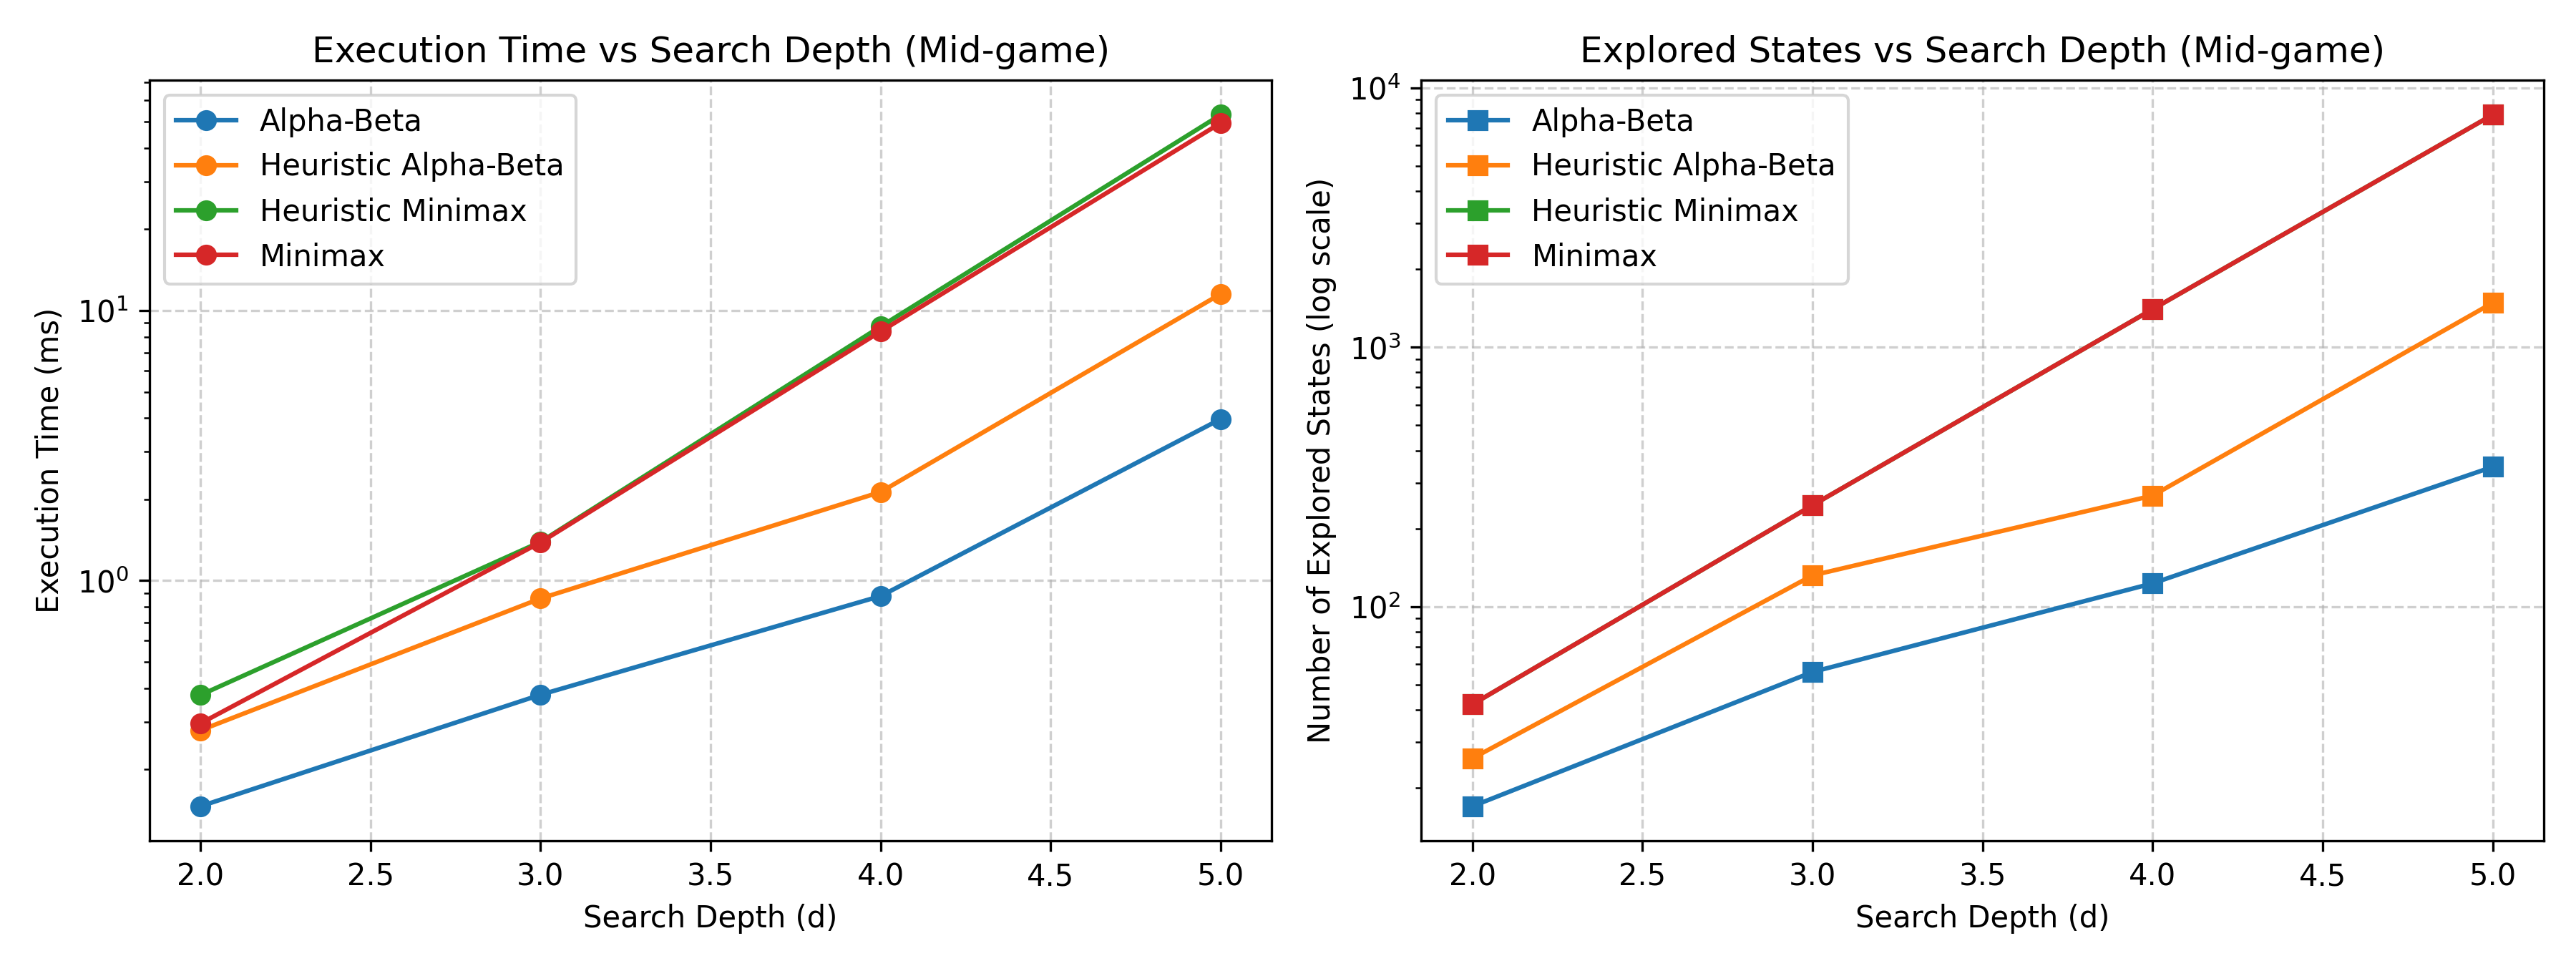
\includegraphics[width=\columnwidth]{task2_benchmark.png}}
\caption{Biểu đồ thời gian thực thi và số trạng thái duyệt theo độ sâu (thang đo logarit).}
\label{fig:task2_bench}
\end{figure}

Từ số liệu ở Bảng~\ref{tab:task2_perf} và Hình~\ref{fig:task2_bench}, có thể rút ra ba nhận xét quan trọng:
\begin{enumerate}
    \item \textbf{Hiệu quả cắt tỉa không gian trạng thái:} Nhờ kết hợp cắt tỉa Alpha-Beta và sắp xếp thứ tự hành động, số lượng trạng thái phải duyệt ở độ sâu $d = 4$ và $d = 5$ giảm từ $75\%$ đến hơn $85\%$ so với duyệt Minimax vét cạn. Ở $d = 5$, H-AB chỉ mất khoảng $26.8\text{ ms}$ cho mỗi lượt đi, hoàn toàn đáp ứng yêu cầu điều khiển xe tăng theo thời gian thực trên giao diện PyGame.
    \item \textbf{Vai trò quyết định của hàm Heuristic:} Minimax thuần và Alpha-Beta thuần trả về giá trị lợi ích bằng $0$ cho mọi trạng thái chưa kết thúc, dẫn đến việc chỉ chọn hành động mặc định đầu tiên trong danh sách. Ngược lại, H-MM và H-AB định hướng xe tăng di chuyển chiến thuật, ngắm bắn và né đạn chính xác.
    \item \textbf{Đối kháng trực tiếp (Bảng~\ref{tab:task2_tour}):} Trong các trận đấu toàn diện trên bản đồ Mid-game và Battle City $13\times 13$, cấu hình H-AB ($d=4$) giành chiến thắng tuyệt đối trước các cấu hình không dùng Heuristic hoặc có độ sâu thấp hơn.
\end{enumerate}

\end{document}